\subsection{Co-Saliency based Palette Generation}
\label{subsec:solver}
On the basis of our co-saliency model we meet DR1 and DR2 by a co-saliency based generation of color palettes %color assignment palette generation.
Taking the model in Eq.~\ref{eq:cosaliency} as the objective within a state-of-the-art color assignment method~\cite{Wang2018}, an optimal color mapping can be obtained from a given  good palette. However, there are two major limitations \od{by not taking palette generation itself into account}: i) the model requires users to try many palettes for selecting a good one; and ii) the design of most existing palettes is not oriented towards visual comparison so that even the best color assignment cannot provide prominent cues for this task.
Fig.~\ref{fig:colorbrewer} shows examples with the Tableau-10 palette and ColorBrewer palette~\cite{harrower2003colorbrewer}. Both results highlight several classes with minor changes (e.g., the bottom left purple class), and make it hard to identify the red class with the largest change  even though it is very distinctive. Thus, we prompt users to use our co-saliency based palette generation method.

%\vspace{1.5mm}
%\noindent\textbf{Co-saliency based Color Assignment}.
%Given a good color palette with $P$ colors ($P\geq M$), the optimal color mapping can be obtained by
%taking the co-saliency model in Eq.~\ref{eq:cosaliency} as the objective of the state-of-the-art color assignment method~\cite{Wang2018}. Starting from a random permutation of $P$ colors, we use the simulated annealing algorithm~\cite{aarts1989stochastic} to find the optimal permutation with two randomized strategies to improve the solution. One is randomly exchanging two colors from the selected $m$ colors and the other is replacing one color from the $m$ selected colors with the one chosen from the unselected $P-M$ colors. With a few iterations, we can obtain a reasonable color mapping as shown in Fig.~\ref{fig:teaser} bottom left.

\begin{figure}[!tb]
\centering
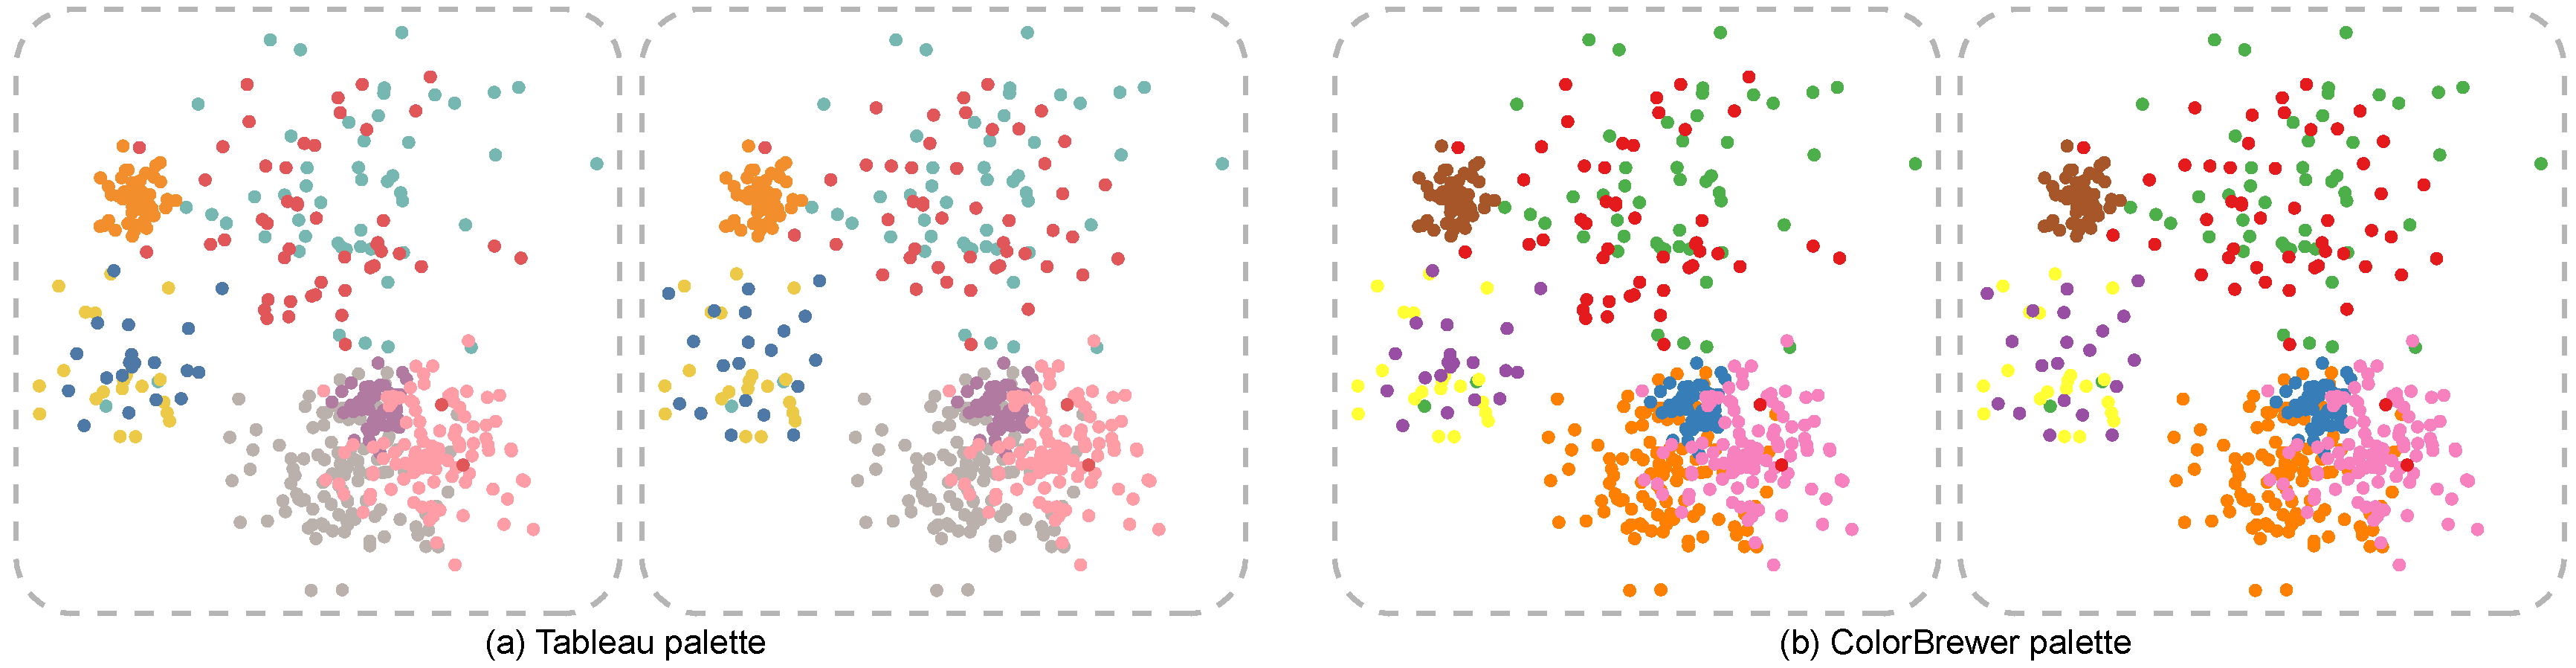
\includegraphics[width=1\columnwidth]{figures/colorbrewer.pdf}
\caption{Results generated by a co-saliency based color assignment with the existing
Tableau-10 palette (a) and the ColorBrewer palette (b). Many existing palettes consist of   bright colors only, where classes with smaller changes cannot be de-emphasized appropriately.}
\vspace*{-3mm}
\label{fig:colorbrewer}
\end{figure}

%However, this method has two major limitations: i) requiring users to try many palettes for selecting a good one; and ii) the design of most existing palettes is not oriented towards visual comparison so that even the best color assignment cannot provide prominent cues for this task.
%For example, all colors in the Tableau palette are highly discriminable and it is hardly to find a satisfactory solution, see Fig.~\ref{fig:teaser} (b). Thus, we prompt users to use our co-saliency based palette generation method.



%\vspace{1.5mm}
%\noindent\textbf{Co-saliency based Palette Generation}.
A recently proposed data-aware palette generation method by Lu et al.~\cite{Lu21} automatically generates discriminable and preferable palettes by maximizing the combination of three palette quality measures: point distinctness, name difference, and color discrimination.
By replacing the first measure with our co-saliency model, palette generation can be formulated as an optimization problem:
\begin{equation}
\arg\max_{\mathbf{\tau}} E(\mathbf{\tau}) = \omega_0 E_{CoS} + \omega_1 E_{ND} + \omega_2 E_{CD}.
\label{eq:energyfunc}
\end{equation}
consisting of a co-saliency term $E_{CoS}$ (see Eq.~\ref{eq:cosaliency}), a name difference term $E_{ND}$ and a color discrimination term $E_{CD}$, balanced by $\omega_0$, $\omega_1$ and $\omega_2$. For more details about $E_{ND}$ and $E_{CD}$, we refer readers to~\cite{Lu21}. By using their optimization method, we are able to generate desired color palettes up to 40 colors in real time. %see Fig.~\ref{fig:teaser} (d).
For example, Fig.~\ref{fig:lambda}(b) shows an example which uses the same dataset as in Fig.~\ref{fig:colorbrewer}, but improves the distinctness of the two changed classes while maintaining class separability.



\subsection{Parameter Effect}
\label{subsec:parameter}
Besides using different weights for the terms in palette generation~\cite{Lu21}, our co-saliency model involves three parameters: the weight $\lambda$ between the two contrasts, the threshold for the class importance $\kappa$, and $\nu$, which is related to the definition of the class change degree that is used as our default class importance.
Since $\nu$ is fixed in our experiments and the class importance can be specified by the user, we mainly discuss here the effects of $\lambda$  and $\kappa$.

\begin{figure}[!htb]
\centering
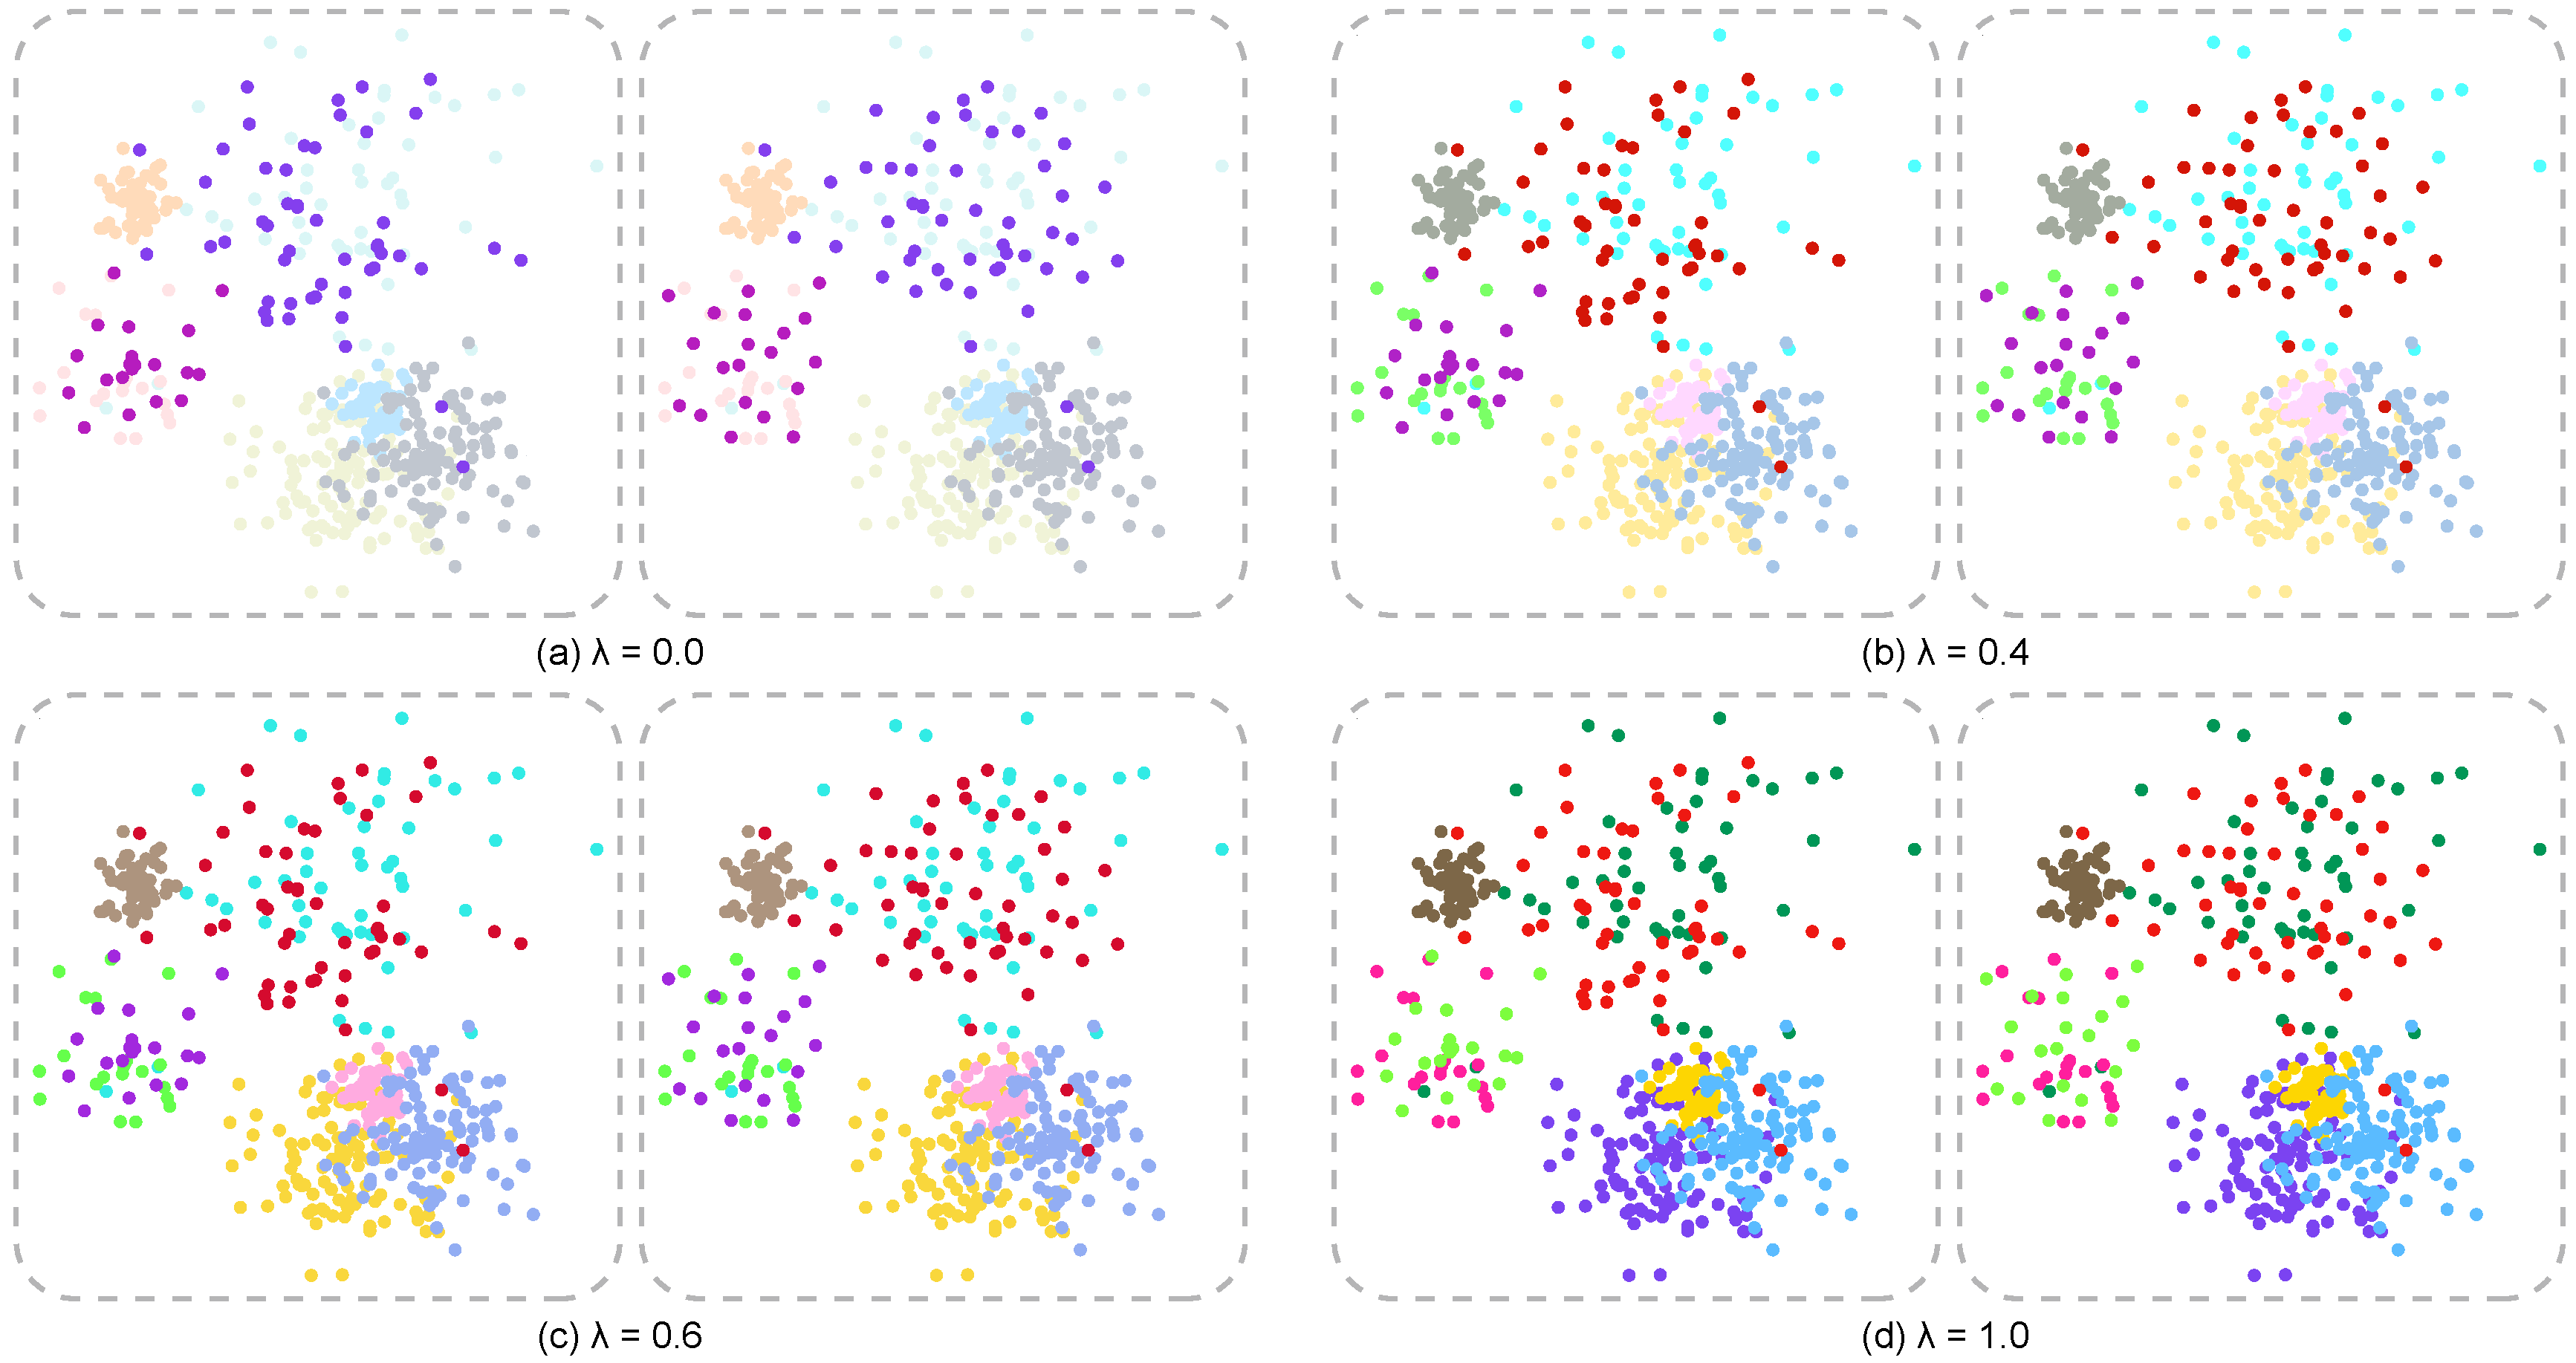
\includegraphics[width=1.0\textwidth]{figures/lambda.pdf}
\caption{Effect of contrast weight $\lambda$: (a) result  considering only contrast to the background; (b) result with $\lambda=0.4$; (c) result with $\lambda=0.6$; (d) result generated by only considering contrast with nearest classes. }
\vspace*{-3mm}
\label{fig:lambda}
\end{figure}
%\vspace{3mm}

\noindent\textbf{Balancing Weight $\lambda$}.
Although this parameter modulates the influence between class contrast with its neighbors and  background, it offers a compromise between DR1 and DR2.
As shown in Fig.~\ref{fig:lambda}(a), considering only the contrast to the background would result in a good 'pop out' effect, but other classes might be hard to discriminate. While considering only the contrast with nearest neighbors, such as done in Fig.~\ref{fig:lambda}(d), all the classes are easy to distinguish but the changed classes are hard to find out.
This is reasonable, because pre-attentive vision
% processing mechanism
lets a bright and saturated color region within regions of de-saturated colors ``pop-out'' to the viewer~\cite{healey1995visualizing}.
In our experiments, we found that setting  $\lambda=0.4$ as a default value allows to simultaneously emphasize changes and preserve the discriminability between classes, see the  example in Fig.~\ref{fig:lambda}(b).

\vspace{1.5mm}
\noindent\textbf{Importance Threshold $\kappa$}.
The importance threshold $\kappa$ selects classes with large importance to be highlighted.
With a default value of zero, all classes with an importance value larger than zero are ensured to be highlighted. Likewise, a large $\kappa$ will de-emphasize classes with a small importance.
We further allow users to specify $\kappa$ by interaction through a widget in our interactive application. %(see Sec.~\ref{sec:interaction}).

%\begin{figure}[h]
%\centering
%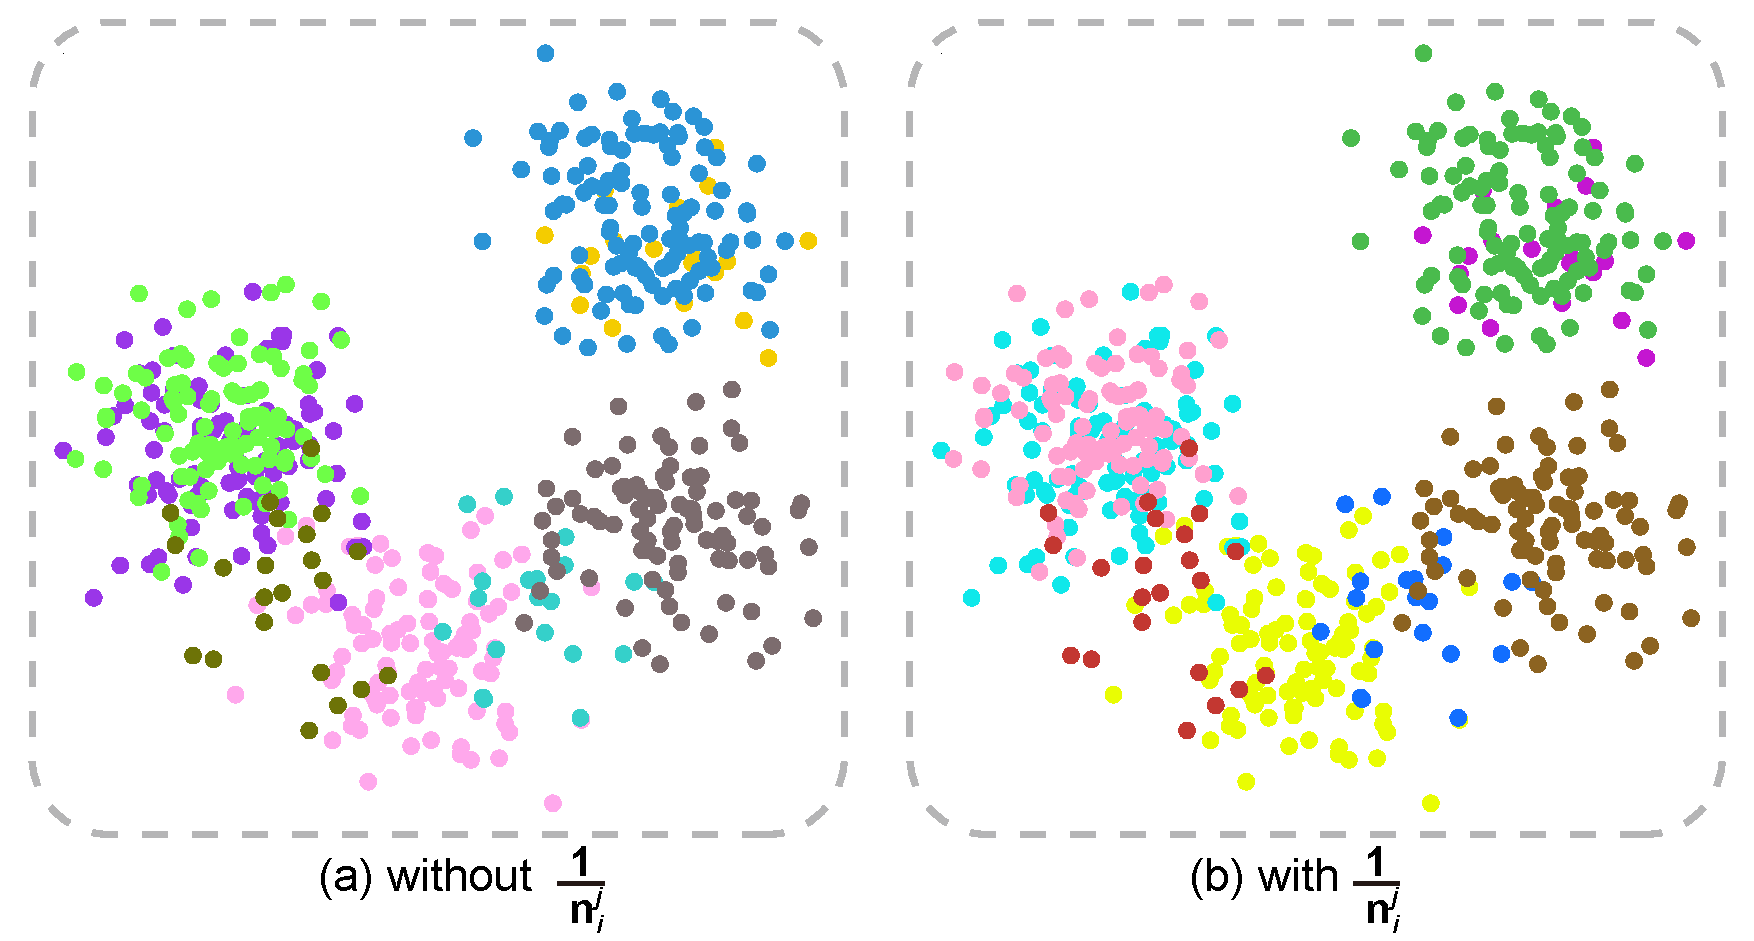
\includegraphics[width=0.8\textwidth]{figures/nij.pdf}
%\caption{Effect of $\frac{1}{n^j_i}$: (a) without this term the small classes are hard to catch user's attention; (b) with this term, small classes are easy to find. Palettes are generated with same scatterplot.}
%\vspace*{-3mm}
%\label{fig:nij}
%\end{figure}
%\vspace{.5em}

%We can observe that when there's only one scatterplot and $\theta_i$ of each class is zero, then Equation.~\ref{eq:cosaliency} is very similar to the objective function of ~\cite{Wang2018}. Our method extends Wang et.al's work to multiple scatterplots with a carefully designed co-saliency model. %Besides, we add $\frac{1}{n^j_i}$ to emphasize the class with less points. As shown in Fig.~\ref{fig:nij}(b), with this new term, the little classes, like red, blue and purple classes, become more discriminable.


\subsection{Bar and Line Charts}
\label{subsec:ext}
%\begin{figure}[t]
%\centering
%\includegraphics[width=0.9\columnwidth]{figures/extensions.pdf}
%\caption{Examples for line graph and bar graph, generated by $\lambda=0.8$ based on Tableau 20.}
%\vspace*{-3mm}
%\label{fig:extension}
%\end{figure}
Like Palettailor~\cite{Lu21}, our color mapping generation method works also for other categorical visualization types such as bar or line charts. This is achieved by treating each bar or line segment in both views as a point and then using the same method to compute their class contrast.
Taking line charts as an example,  we order the line segments along the time axis and build a one-to-one mapping for line segments to compute $\theta_i$.
Doing so, lines with large changes will be highlighted while maintaining the discriminability between multiple lines in each chart. The same is done for bar charts, see Fig.~\ref{fig:teaser}.
%Fig.~\ref{fig:extension} shows our color palette generation results on line charts, where the red and blue lines are highlighted while maintaining the discriminability between multiple lines in each chart.
More results can be found in our supplementary material.

